\chapter{Testy wydajności}
Poniżej przedstawione zostały zaimplementowane testy wydajności wraz z krótkim opisem, porównaniem działania między systemami testowymi oraz analizą z czego wynikają ograniczenia wydajności.

\section{Test oświetlenia}
W ramach tej sekcji sprawdzone zostały możliwości modułu w aspekcie obsługi dużej ilości źródeł światła. Nie używając zmodyfikowanej techniki forward rendering limitem jest około 1300 świateł, bez względu na wydajność takiej aplikacji. Wartością testowaną jest w tym przypadku ilość źródeł światła. Poniżej przedstawione zostały użyte parametry oraz wyniki.

\begin{center}
	\begin{tabular}{ |l r|}
		\hline
		\textbf{Parametr} & \textbf{Wartość} \\
		\hline
		Target FPS & \textbf{60} \\
		Target curve multiplier & \textbf{0.75} \\
		Rozdzielczość & \textbf{1920x1080} \\
		\hline
	\end{tabular}
	\quad
	\begin{tabular}{ |l r|}
		\hline
		\textbf{Układ graficzny} & \textbf{Ilość źródeł światła} \\
		\hline
		NVIDIA 4060 & \textbf{1647} \\
		Radeon 780M & \textbf{934} \\
		\hline
		Procent wydajności & \textbf{56.71\%} \\
		\hline
	\end{tabular}
\end{center}

W trakcie testu zużycie obu GPU oscylowało w graniach 95\%-100\%, co w połączeniu z relatywnie dużym spadkiem wydajności między układami oraz specyfiką badanego obszaru wskazuje na ograniczenie ze strony mocy układu graficznego. 

Do poprawy wydajności należałoby podejść od strony optymalizacji techniki rysowania świateł. Forward rendering nie jest najlepszą techniką przy tak dużej ilości źródeł światła i w przypadku takiego wymogu lepszym podejściem byłoby zastosowanie Deferred Shading. 

Zrzut ekranu ze stanu wyświetlania po osiągnięciu zadanego celu wydajnościowego został przedstawiony na rys. \ref{demo_test_lights}.

\vfill

\begin{figure}[h!]
	\centering
	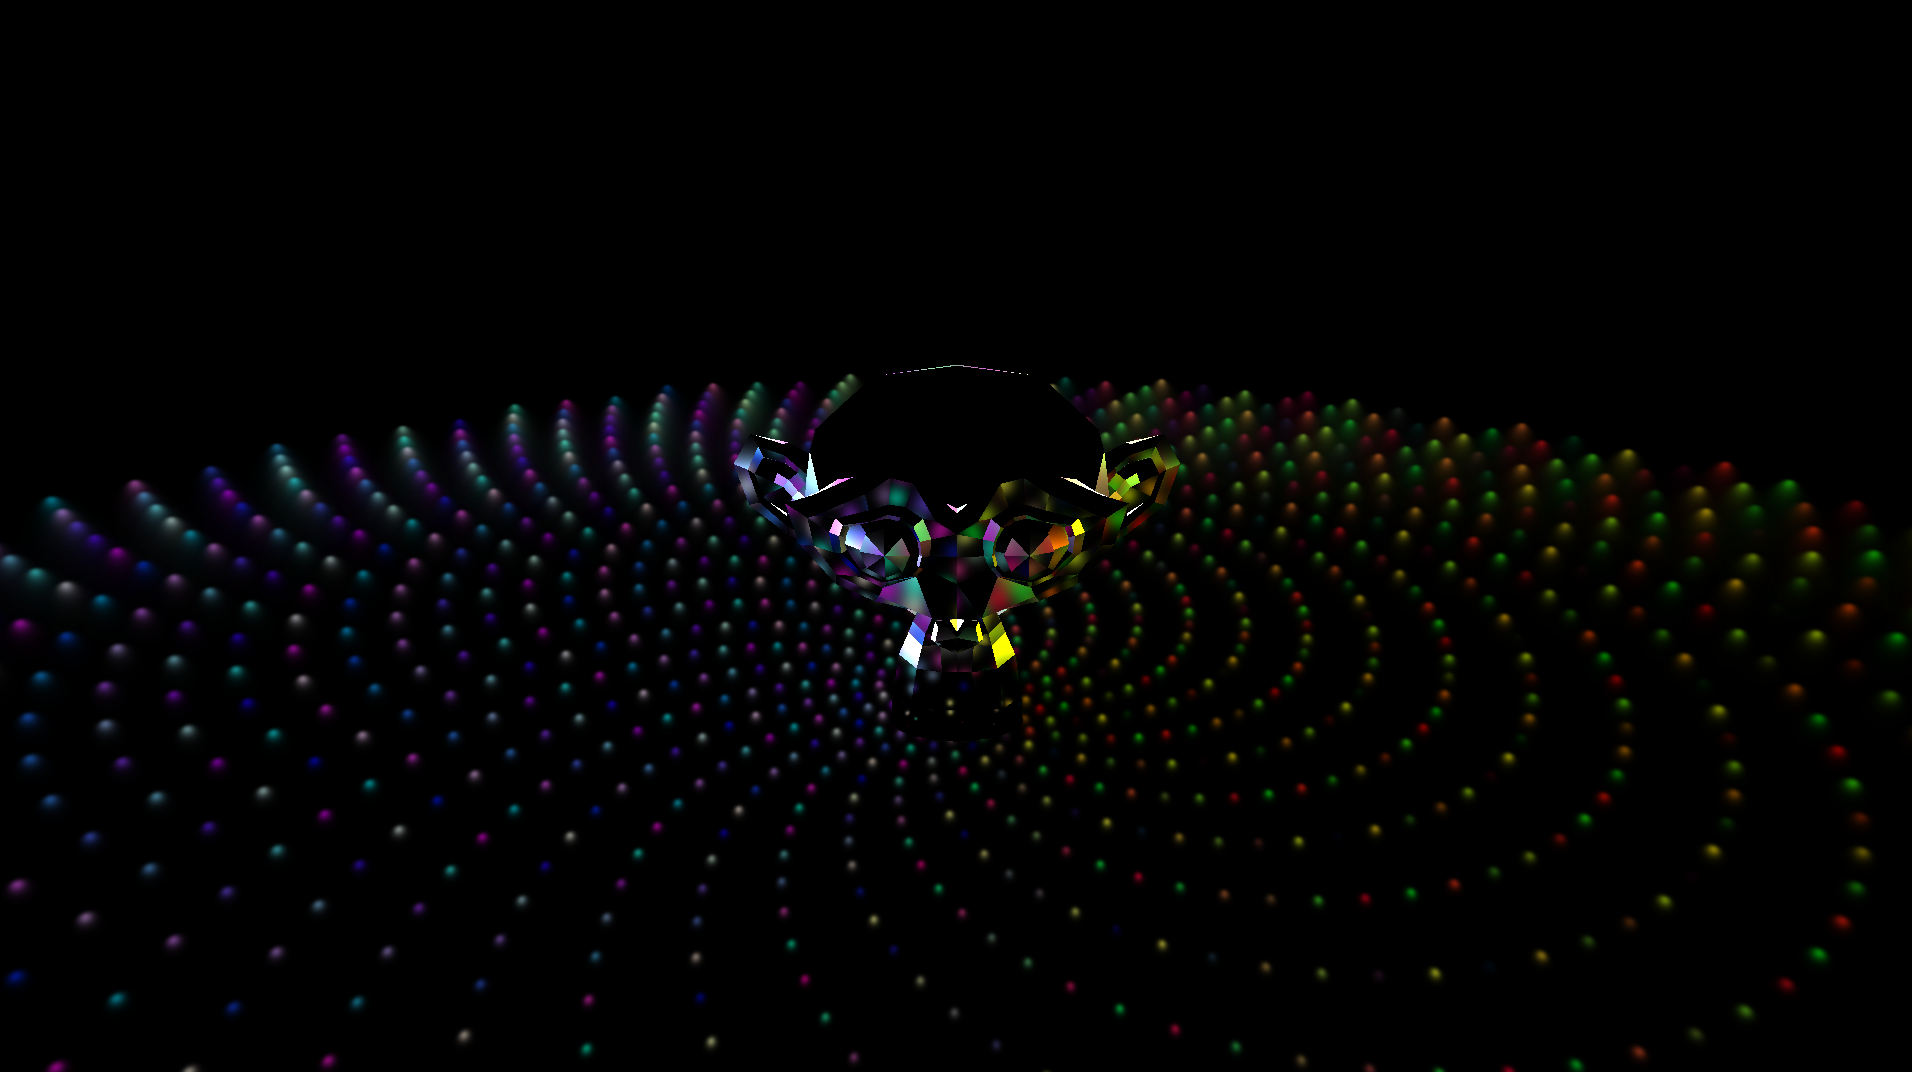
\includegraphics[width=\textwidth]{images/demo_test_lights.png}
	\caption{Zrzut ekranu przedstawiający test oświetlenia z aktywnymi 1647 źródłami światła.}
	\label{demo_test_lights}
\end{figure}

\section{Test wielu obiektów}
\label{section_test_multilpe_objects}
Druga sekcja skupia się na możliwości przetwarzania wielu modeli na ekranie jednocześnie. Taki test sprawdza wydajność prawie każdej części procesu renderowania - od optymalizacji zmian kontekstu, przez ilość danych przesyłanych po magistrali, a kończąc na wydajności programów przetwarzania wierzchołków i cieniujących. Obraną wartością testową jest ilość niezależnych obiektów, będących prostymi modelami sześcianu. Wszystkie stworzone elementy są cały czas widoczne na ekranie, choć w bardzo małej skali. Poniżej pokazane zostały standardowe parametry oraz wyniki.

\begin{center}
	\begin{tabular}{ |l r|}
		\hline
		\textbf{Parametr} & \textbf{Wartość} \\
		\hline
		Target FPS & \textbf{60} \\
		Target curve multiplier & \textbf{0.05} \\
		Rozdzielczość & \textbf{800x800} \\
		\hline
	\end{tabular}
	\quad
	\begin{tabular}{ |l r|}
		\hline
		\textbf{Układ graficzny} & \textbf{Ilość obiektów} \\
		\hline
		NVIDIA 4060 & \textbf{14370} \\
		Radeon 780M & \textbf{9341} \\
		\hline
		Procent wydajności & \textbf{65.00\%} \\
		\hline
	\end{tabular}
\end{center}

W trakcie wykonywania testu można było zaobserwować niskie zużycie GPU, około 15\%, a także wysoki procent obciążenia procesora centralnego, w szczególności pojedynczego rdzenia. Względnie duża różnica między wynikami sugeruje jednak także duży udział układu graficznego w ograniczeniu wydajności. 

W celu poprawy wydajności w pierwszej kolejności poprawie powinien zostać poddany moduł generujący zapytania do API tak, aby dodać wsparcie wielowątkowości. Ograniczenie złożoności shader'a przetwarzania wierzchołków także pomogłoby w poprawie wyniku.

Test pokazuje także skuteczność działania AssetManager'a. Pierwsze wczytanie modelu zajęło \textbf{1048ms}, a każde kolejne mniej niż \textbf{0.001ms}.

Zrzut ekranu finalnego stanu testu przedstawiony został na rys. \ref{demo_test_objects}.

\begin{figure}[h!]
	\centering
	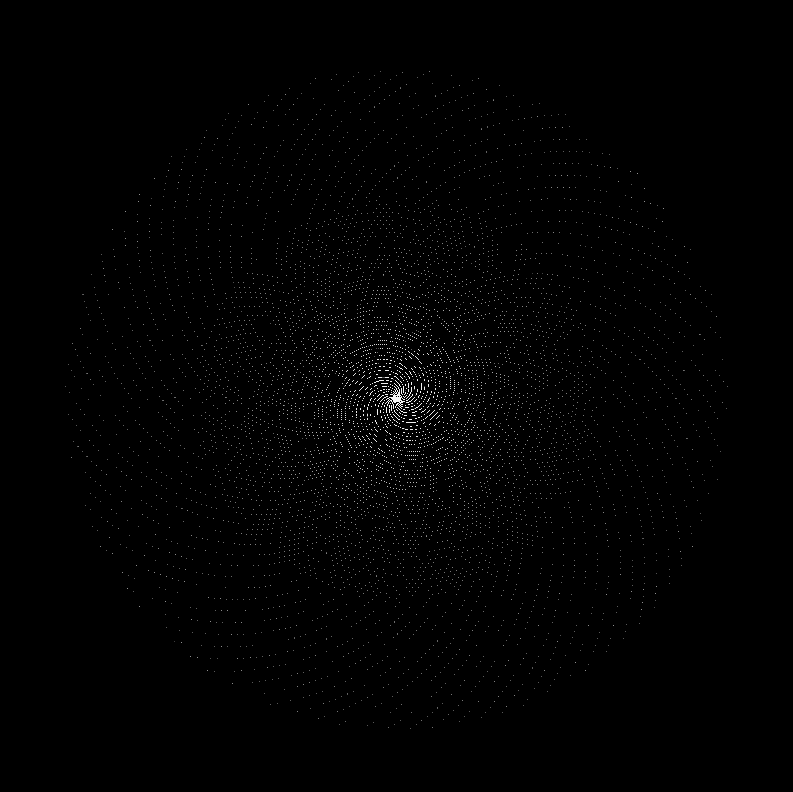
\includegraphics[width=0.55\textwidth]{images/demo_test_objects.png}
	\caption{Zrzut ekranu przedstawiający 14370 jednocześnie wyświetlanych obiektów.}
	\label{demo_test_objects}
\end{figure}

\section{Test wydajności modułu Transform}
W przypadku pomiaru limitów ważnym jest także określenie maksymalnej ilości obiektów w hierarchii sceny. Przy opisywaniu poprzednich rozdziałów przedstawiona została klasa Transform, odpowiedzialna za zachowywanie wzajemnych relacji transformacji między obiektem rodzicem, a jego dziećmi. Opisywany test wykonuje próbę oszacowania teoretycznej maksymalnej ilości obiektów z założeniem modyfikacji transformacji głównego rodzica raz na klatkę obrazu. W tym celu tworzona jest struktura drzewowa o określonej maksymalnej szerokości, kontrolowanej przez parametr \textbf{mElementsPerLevel} o domyślnej wartości 5000. Po przekroczeniu tej ilości w ramach jednego poziomu kolejne obiekty dodawane są do ostatniego elementu poprzedniego stopnia, aż do powtórzenia się sytuacji. Następnie taka struktura poddawana jest testowi przez zmianę rotacji obiektu głównego, co powoduje także aktualizację transformacji obiektów podległych. Aby oddać rzeczywiste ograniczenia bez zmian pozostała cała reszta modułu, ale w celu zmniejszenia obciążenia GPU obiekty nie są wyświetlane na ekranie, a rozdzielczość jest bardzo niska. Pełne parametry jak i wyniki przedstawione zostały poniżej.


\begin{center}
	\begin{tabular}{ |l r|}
		\hline
		\textbf{Parametr} & \textbf{Wartość} \\
		\hline
		Target FPS & \textbf{60} \\
		Target curve multiplier & \textbf{0.1} \\
		Rozdzielczość & \textbf{256x256} \\
		\hline
	\end{tabular}
	\quad
	\begin{tabular}{ |l r|}
		\hline
		\textbf{Układ graficzny} & \textbf{Ilość obiektów} \\
		\hline
		NVIDIA 4060 & \textbf{110407} \\
		Radeon 780M & \textbf{97083} \\
		\hline
		Procent wydajności & \textbf{87.93\%} \\
		\hline
	\end{tabular}
\end{center}


W trakcie wykonywania testu obciążenie GPU nie przekraczało 2\%, co zgodnie z oczekiwaniami sugeruje ograniczenie po stronie procesora głównego. Spadek około 12\% na zintegrowanym układzie graficznym wynika prawdopodobnie ze zmniejszonego poboru mocy procesora ze względu na dzielenie jej z GPU, a co za tym idzie ze zmniejszonej częstotliwości taktowania CPU.

Optymalizacja tej sekcji tak jak poprzedniej opierałaby się w większości na dodaniu obsługi wielowątkowości, choć ze względu na charakterystykę procesu mogłoby to być mniej skuteczne niż w przypadku zapytań API. Możliwym byłoby także częściowe przeniesienie obliczeń związanych z transformacjami na GPU w ramach shader'a przetwarzania wierzchołków. Takie podejście zmniejszyłoby jednak wydajność układu graficznego, a to jest koszt, który w praktycznych zastosowaniach rzadko jest ostatecznie korzystny. 

\section{Test przetwarzania wierzchołków}
Ostatnią zaimplementowaną na bazie \textit{AutoTest} sekcją jest test określający teoretyczny limit ilości przetwarzanych i wyświetlanych wierzchołków. Ustalenie tej wartości jest jednak trudne, ze względu na jej częste powiązanie z wydajnością przetwarzania wielu obiektów, czego test został opisany w ramach sekcji \ref{section_test_multilpe_objects}. Aby uniknąć tego ograniczenia użyty został pojedynczy model, składający się z bardzo dużej ilości wierzchołków, a dokładniej \textbf{Roman Marble Ornate Plinth} ze zbioru Quixel Megascans \cite{fab:QuixelMegascans:RomanMarbleOrnatePlinth}, składający się z 3 milionów wierzchołków. Przy wczytywaniu danych biblioteka assimp dokonuje automatycznej optymalizacji, przez co finalną wartością jest 1.5 miliona. Jako testowaną wartość przyjęta została ilość wyświetlanych modeli, a wynik pomnożony zostaje przez 1.5 miliona, celem uzyskania całkowitej sumy wyświetlanych vertex'ów. Parametry oraz wyniki zostały pokazane poniżej, a zrzut ekranu przedstawiający stan na końcu testu na rys. \ref{demo_test_vertex}.

\begin{center}
	\begin{tabular}{ |l r|}
		\hline
		\textbf{Parametr} & \textbf{Wartość} \\
		\hline
		Target FPS & \textbf{60} \\
		Target curve multiplier & \textbf{0.5} \\
		Rozdzielczość & \textbf{640x480} \\
		\hline
	\end{tabular}
	\quad
	\begin{tabular}{ |l r|}
		\hline
		\textbf{Układ graficzny} & \textbf{Ilość wierzchołków} \\
		\hline
		NVIDIA 4060 & \textbf{12072936} \\
		Radeon 780M & \textbf{3018234} \\
		\hline
		Procent wydajności & \textbf{25.00\%} \\
		\hline
	\end{tabular}
\end{center}

\vfill
\clearpage

\begin{figure}[h!]
	\centering
	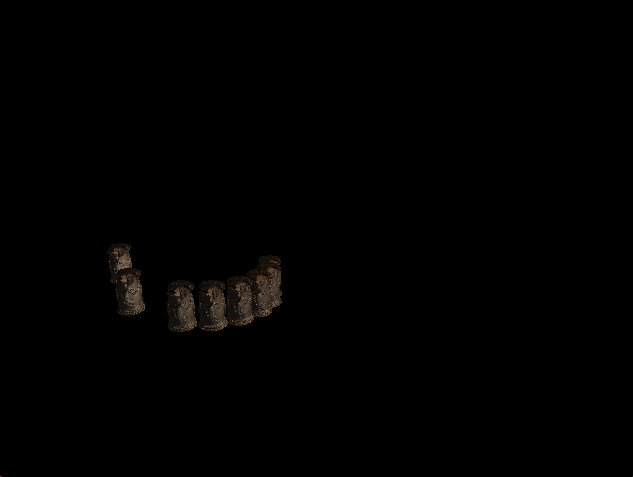
\includegraphics[width=0.55\textwidth]{images/demo_test_vertex.png}
	\caption{Zrzut ekranu pokazujący 8 obiektów o łącznej sumie wierzchołków liczącej 12072936.}
	\label{demo_test_vertex}
\end{figure}

W ramach testu wystąpiła największa różnica między układami graficznymi. Wynika ona najprawdopodobniej z przewagi układu dedykowanego na płaszczyźnie przepustowości oraz opóźnień pamięci. O ile wykorzystywana przez iGPU LPDDR5x charakteryzuje się bardzo dobrymi parametrami w kontekście pamięci głównej systemu, to nie można jej stawiać w jednym szeregu z dedykowaną pamięcią GDDR6 wykorzystywaną z kartą NVIDIA RTX 4060, co jest szczególnie widoczne przy obsłudze tak dużej ilości wierzchołków. Wysokie obciążenie pamięci w ramach testu udało się potwierdzić poprzez manipulację taktowaniem dedykowanego układu graficznego. Zmniejszenie częstotliwości pracy rdzenia o \textbf{20\%} - z 2500MHz na 2000MHz - skutkowało spadkiem wydajności tylko o \textbf{10\%}. W kontraście obniżenie taktowania pamięci zaledwie o \textbf{6.25\%} - z 8000MHz na 7500MHz, czyli minimalną możliwą do ustawienia wartość - skutkowało spadkiem wyniku aż o \textbf{15\%}.
